%! TEX root = ./main.tex

\lecture{21}{Week: 11}{Continue: Virtual Memory}

\paragraph{Terminology}
\textit{Virtual Page} may refer to a page-aligned region of virtual memory space or to the content of this region. The \textit{Physical Page} reverse to a page-aligned region in physical memory. The \textit{Physical Frame} is the container of the page.

\subsubsection{Multi-Level Page Tables}

\paragraph{Motivation: Linear Page Table Size}
Given:
\begin{itemize}
    \item $4$ KB page size
    \item $48$-bit address space
    \item $8$-byte PTE
\end{itemize}

The resulting page table has size: $\#\text{PTE} \cdot \text{PTE size}$ and the number of PTE is $\text{address space size} / \text{page size}$. This gives $2^{48} / 2^{12} \cdot 2^3 = 2^{39} \text{bytes} = 512 \text{GB}$.

This page table would never fit into memory. To reduce this size, we use additional levels of indirections.

\paragraph{Two Level Page Table Hierarchy}
In this setup, we have two page tables. Lable one contains the full range of virtual addresses. In contrast to that, the second level tables are only created when needed. When we access not previously accessed page table, an entry in the PT1 is created, and its entry points to the base address of the table of the second page table. The second page table entry does then point to the actual PTE from where we can get the PPN.

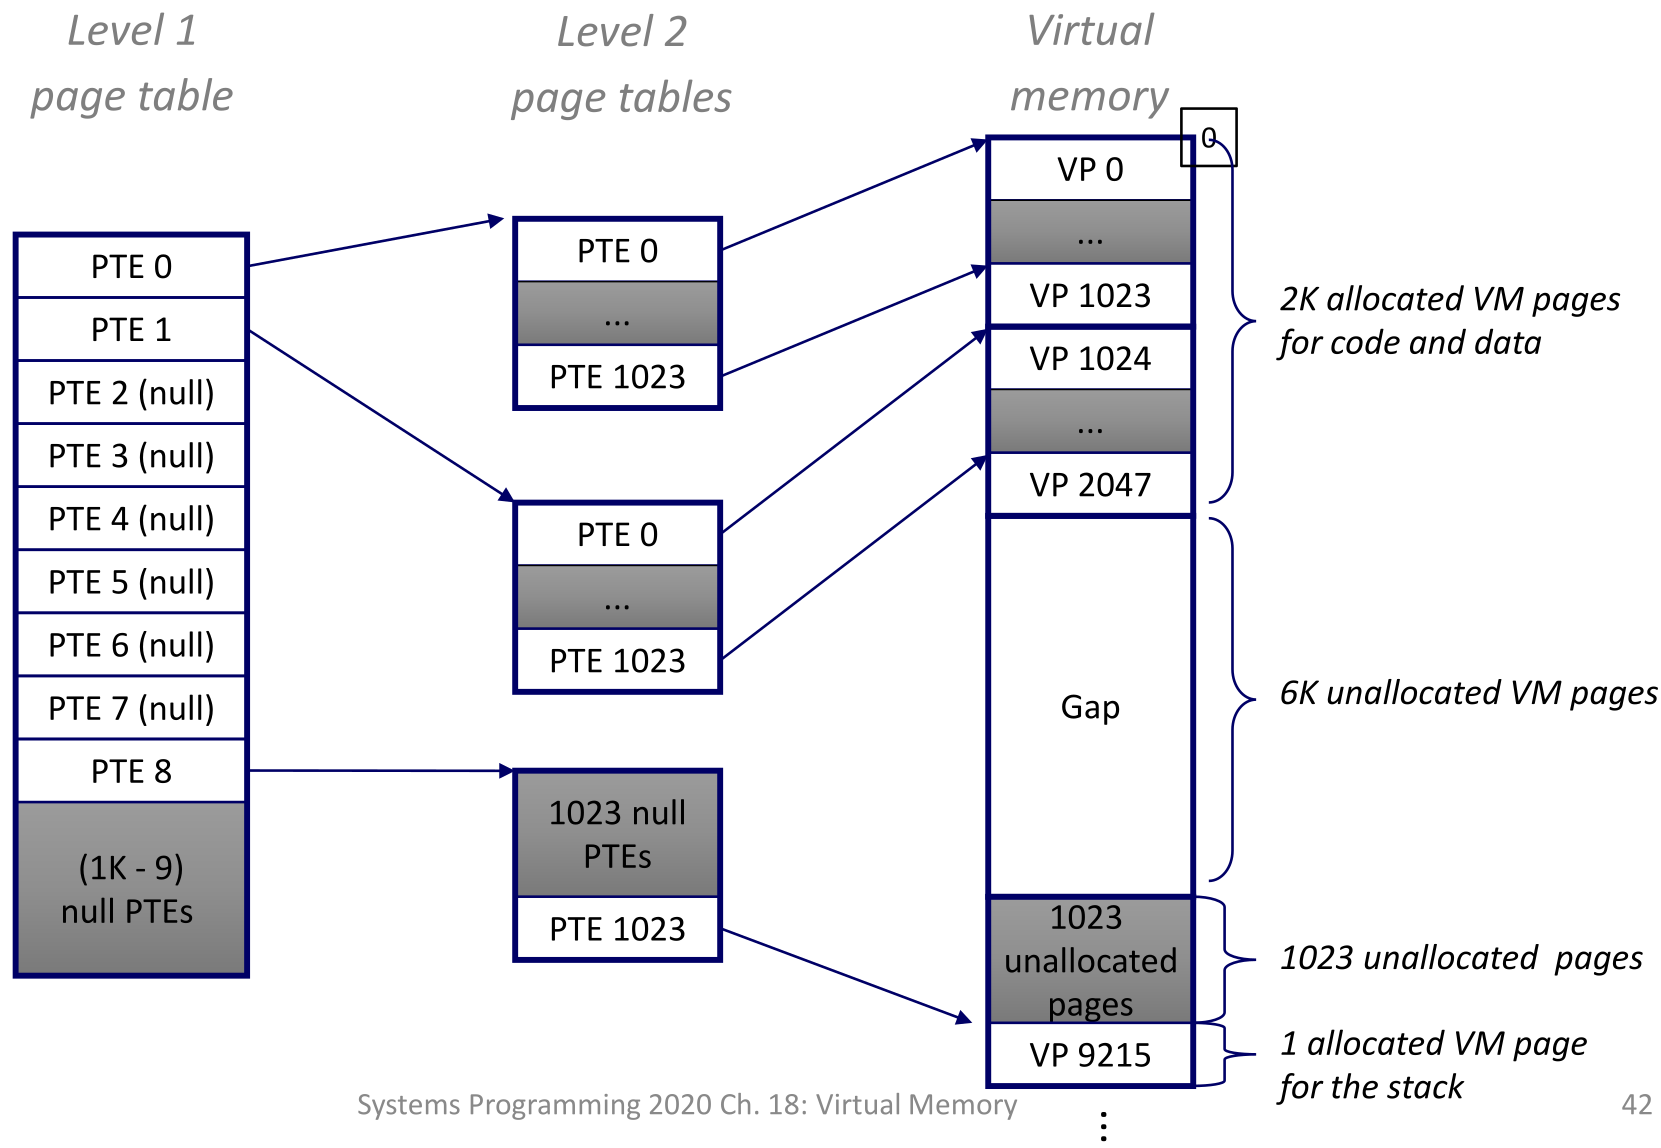
\includegraphics[width=0.8\textwidth]{21_2LayerPT.png}

The page tables of the different levels are induced by different parts of the VPN. This concept can easily be extended to $k$ levels. In x86-64 $4$ layers of indirection.

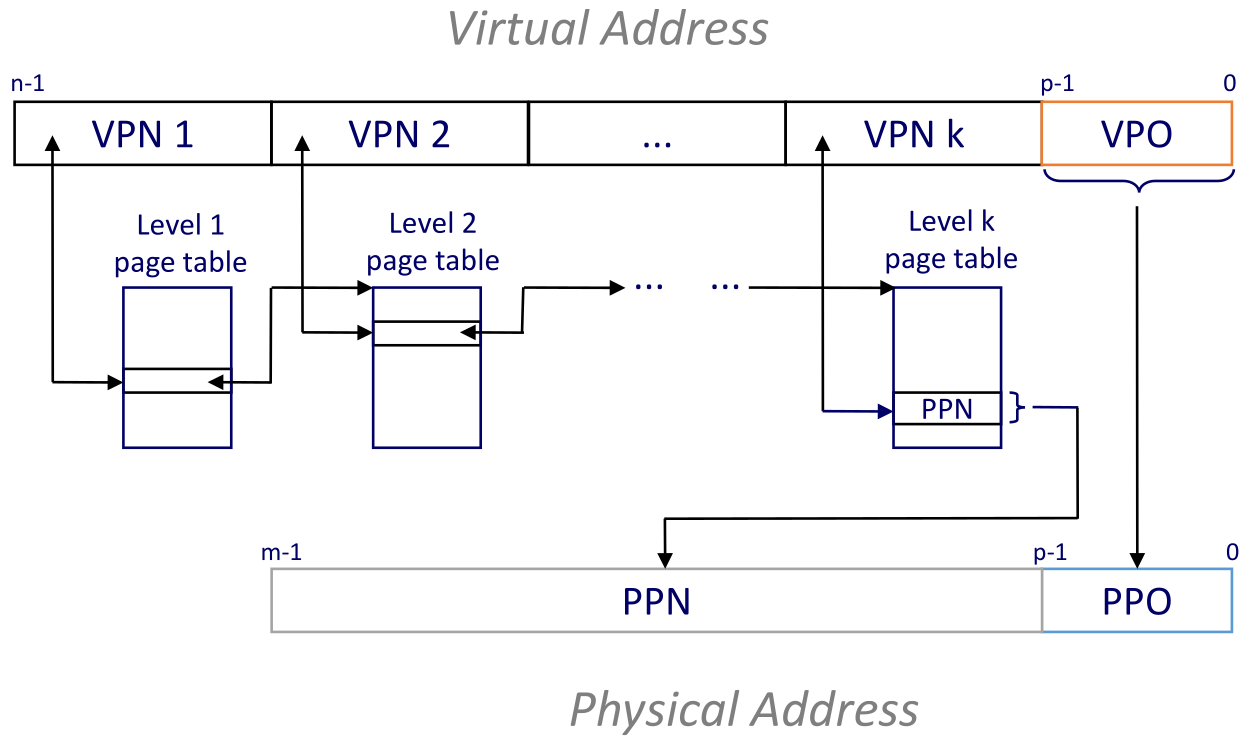
\includegraphics[width=0.8\textwidth]{21_kLayerPT.png}

As long as we get a hit in page table $i-1$ we can index into page table $i$.

\subsubsection{Case Study: i7}
A typical i7 processor has the following CPU schema:

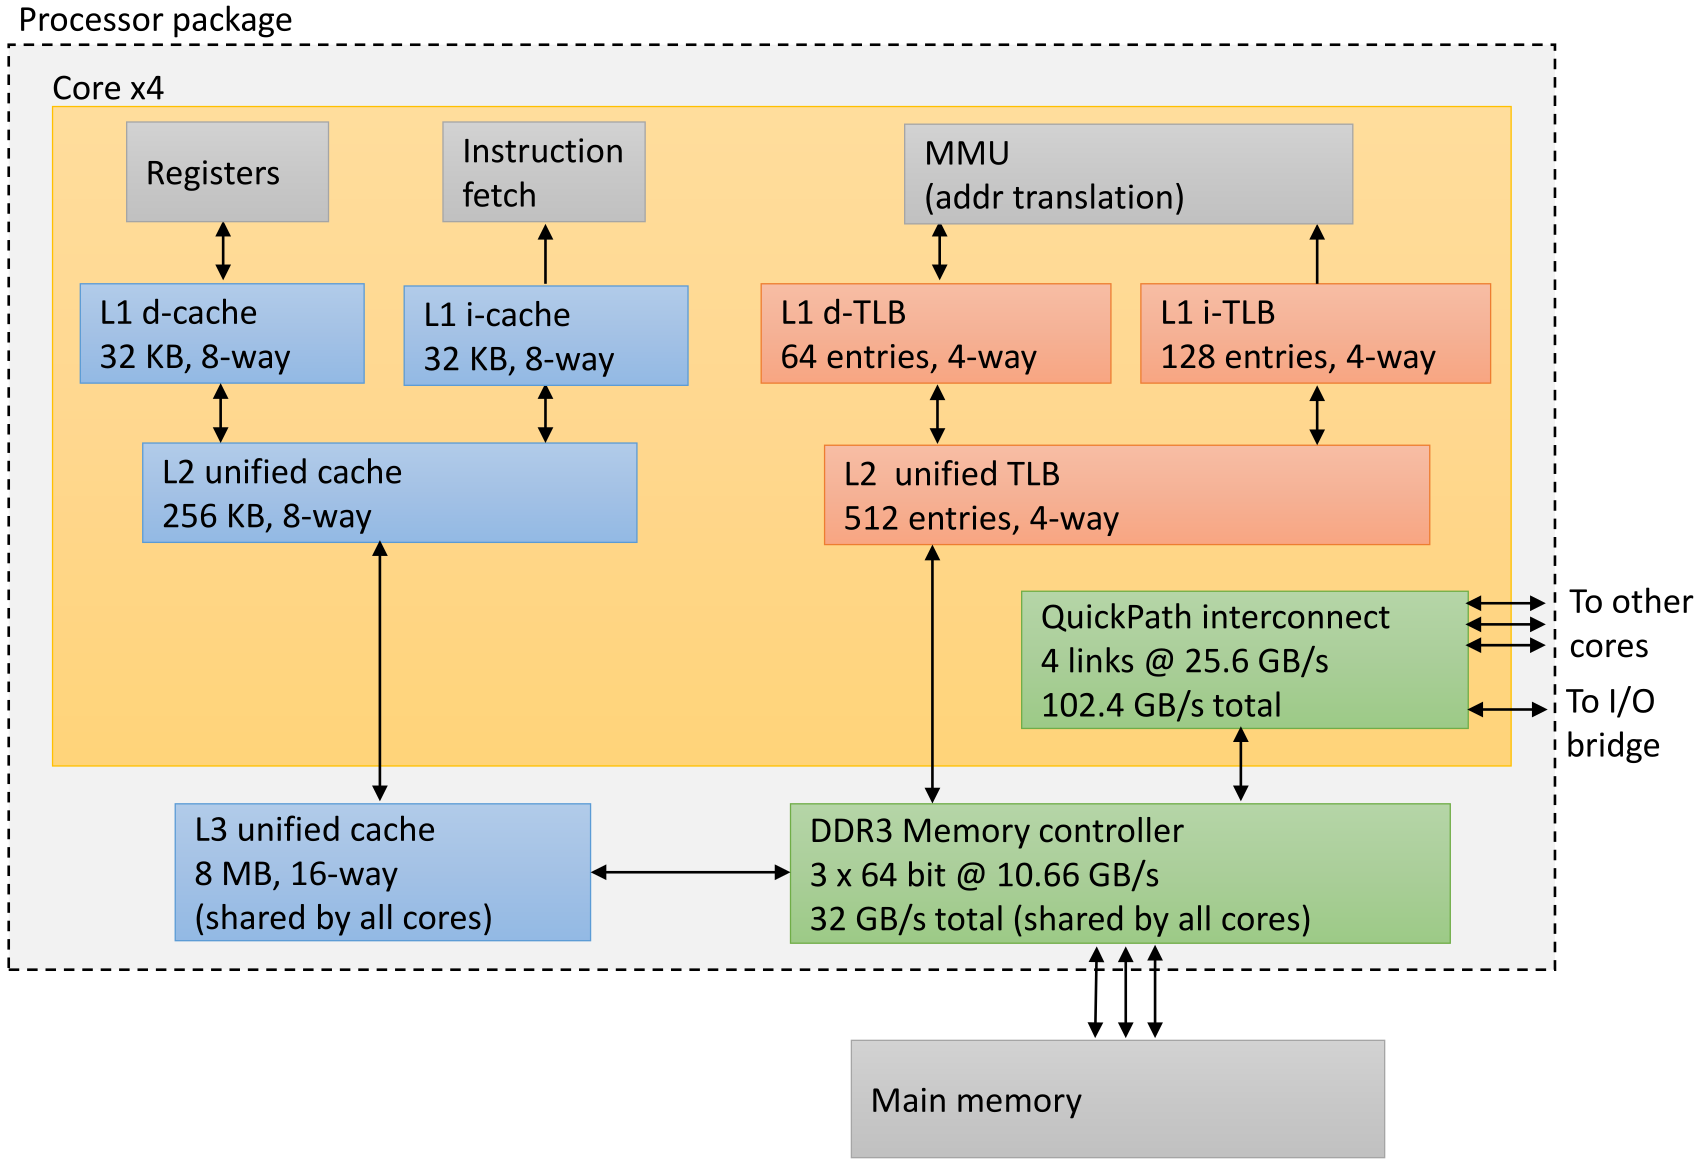
\includegraphics[width=0.8\textwidth]{21_i7CpuSchema.png}

And the following memory system:

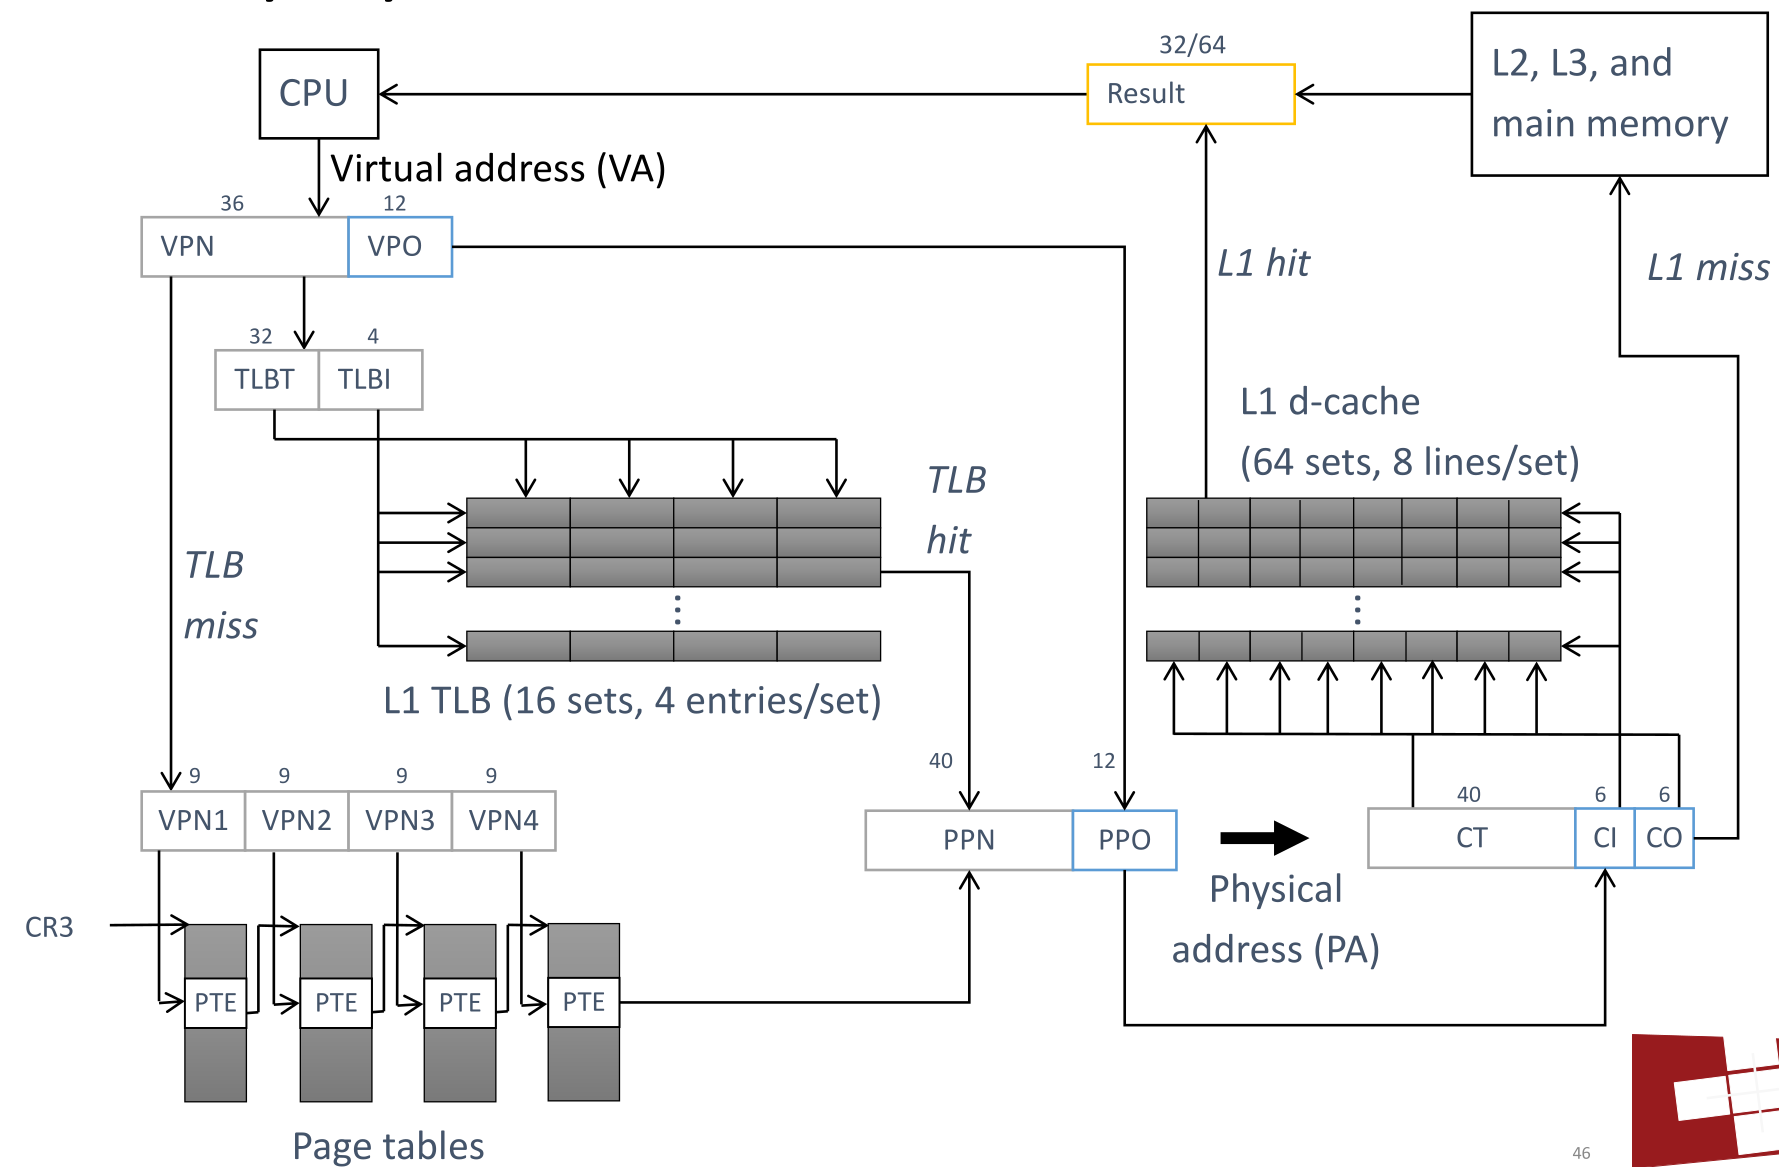
\includegraphics[width=0.8\textwidth]{21_i7MemorySystem.png}

The \code{CR3} is the register which hold the process specific base address of the page table.

The VA has typically $48$ bit size and the PA is $52$ bits. The PPN has to be $40$ bits long and hence, a table entry must be $64$ bits.

\paragraph{TLB}
This part of the CPU is poorly documented and includes speculations.

A TLB entry is $77$ bits long and contains beside the PPN and the TLBT, also a few flags. It is important that the PTE contains also the permissions bits.

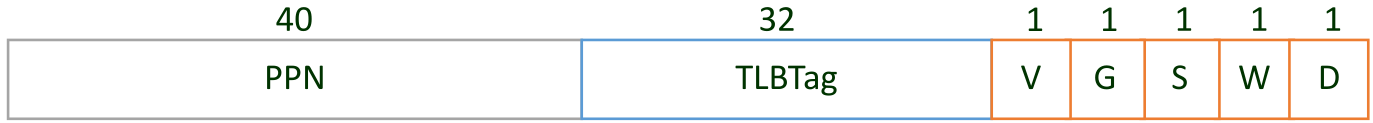
\includegraphics[width=0.8\textwidth]{21_i7Tlb.png}

\begin{description}
    \item[V:] valid bit determines if this entry contains valid data.
    \item[TLBT:] is used to match and check if this is the right entry.
    \item[PPN:] the address we are looking for.
    \item[G:] global bit tells if page is global or not (Global tables are not evicted on content switch).
    \item[S:] supervisor flag tells if page is accessible by superuser only.
    \item[W:] writ flag.
    \item[D:] dirty bit tells if data of this page was modified and requires writeback to memory.
\end{description}

The TLB is structured as $16$ sets with $4$ entries. The $4$ entries are used to cache the entries of the $4$ layers.

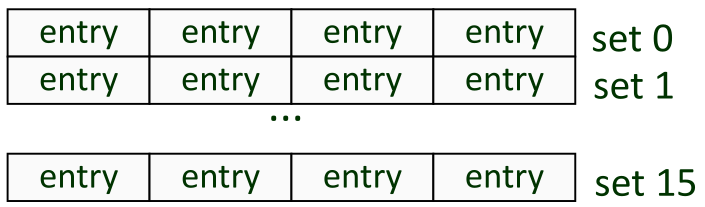
\includegraphics[width=0.8\textwidth]{21_i7TlbStructure.png}

\paragraph{Paging}
\textit{Paging} or \textit{page walk} is the process of going though the different levels of the tage tables. In i7 the $4$ tables have different names and are numbered in decreasing order starting with the \textit{first} table.

All $4$ tables have a entry size of $64$ bits.

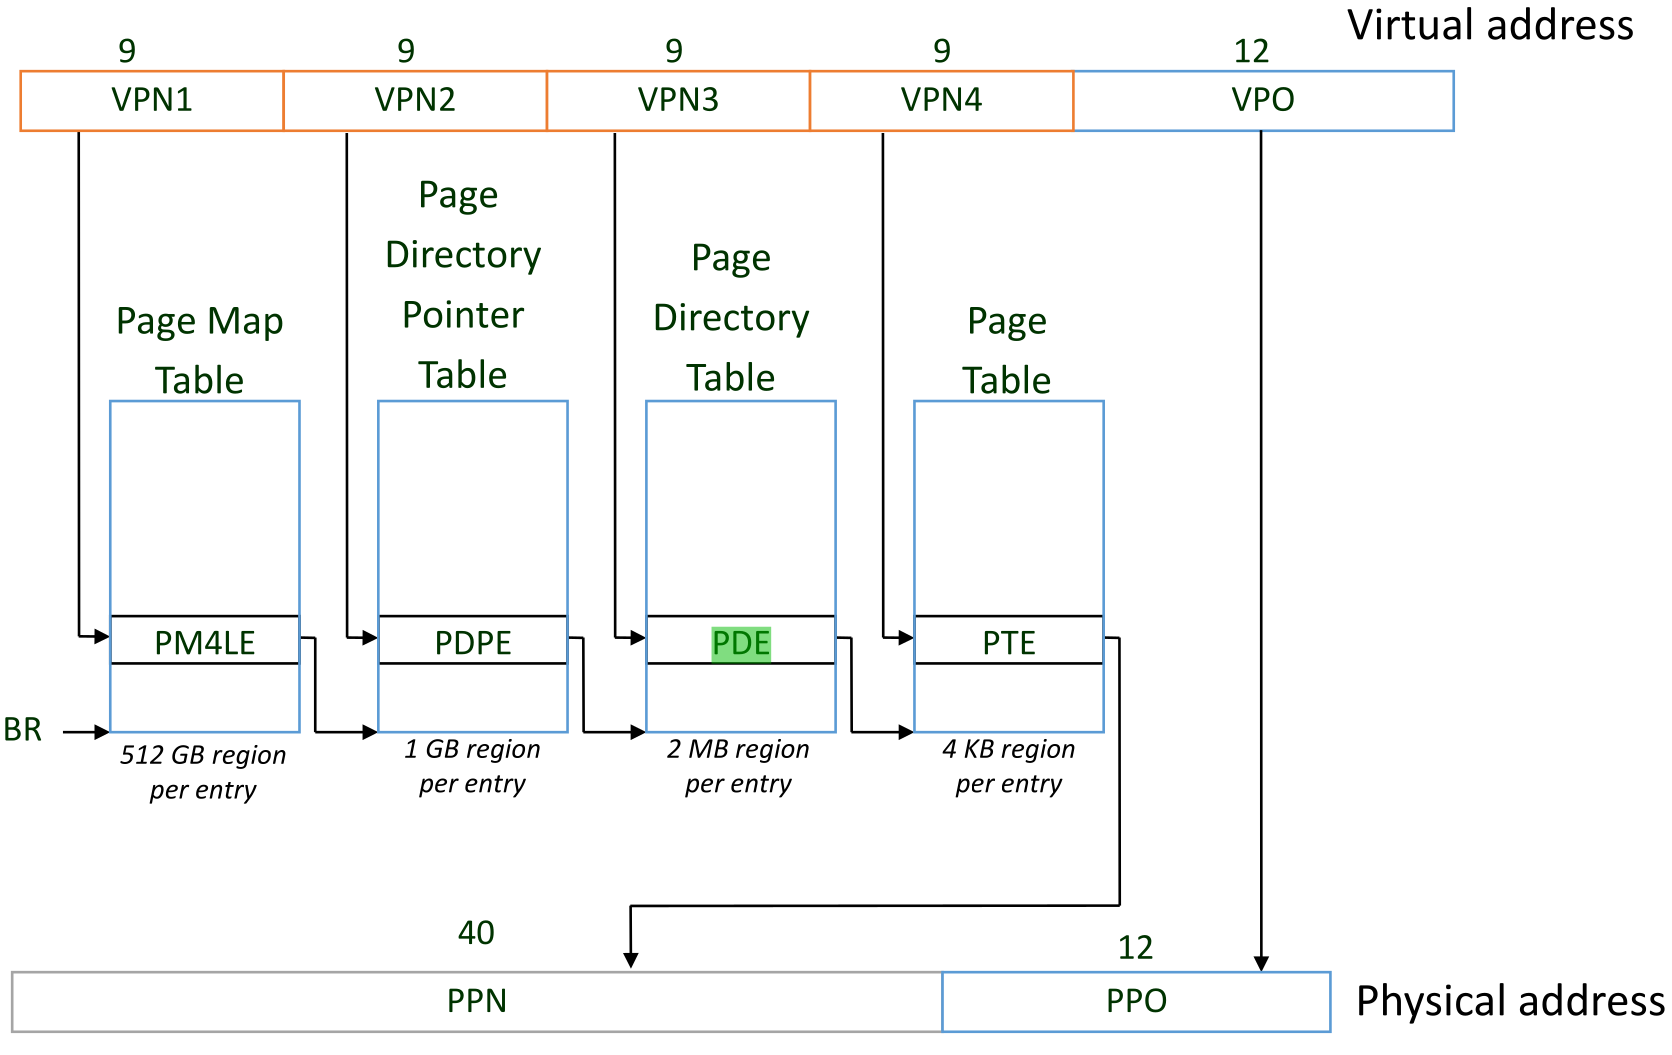
\includegraphics[width=0.8\textwidth]{21_i7Paging.png}

\subparagraph{Level 4: Page Map Table}
This is the \textit{first} table in the hierarchy.

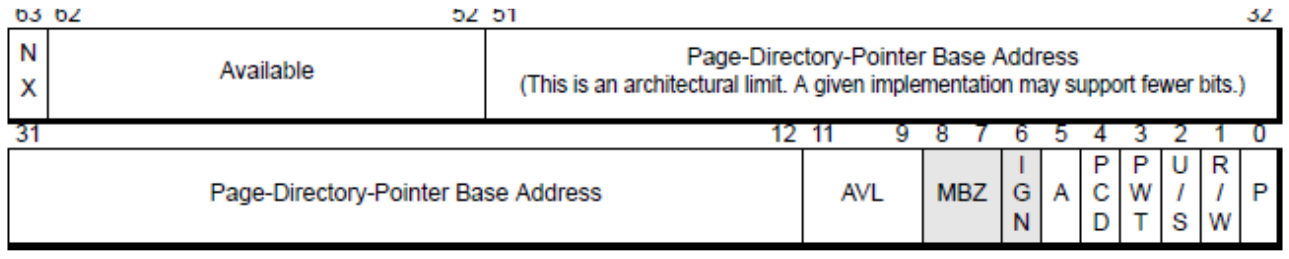
\includegraphics[width=0.8\textwidth]{21_i7L4.png}

\begin{description}
    \item[Page Directory Pointer Base Address:] $40$ MSB are the pointer to the base address of level 3
    \item[Avail:] Bits available to programmers for testing
    \item[A:] access bit is set by the MMU on a read or write. Periodically, it is reset by a OS process. This way we can determine less frequently used entries.
    \item[PCD:] is used to tell if a page should be cached or not.
    \item[PWT:] determines if we use write-through or write-back cache policy for this table.
    \item[U/S:] determine is table belongs to user or supervisor mode.
    \item[R/W:] determine read-only or read-write access
    \item[P:] flag which tells if page table is present in memory or not.
\end{description}

\subparagraph{Level 3: Page Directory Pointer Entry}
Is appointed by the Page Map Table.

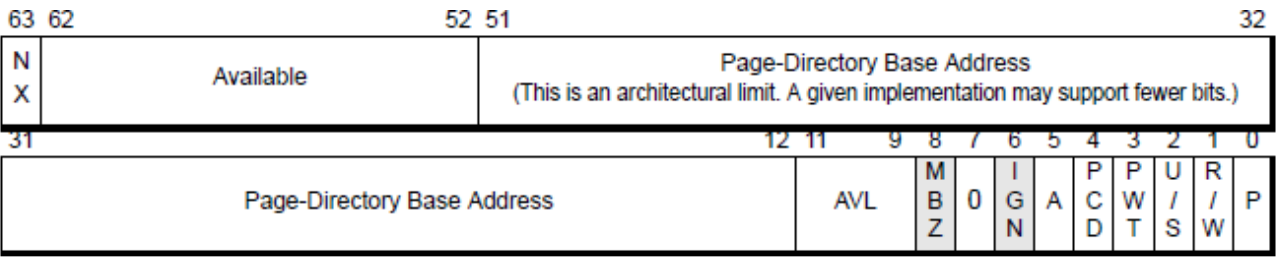
\includegraphics[width=0.8\textwidth]{21_i7L3.png}

\begin{description}
    \item[Page Directory Base Address:] $40$ MSB are the pointer to the base address of level 2
\end{description}

All other parts of the entry are equivalent to level 4.

\subparagraph{Level 2: Page Directory Entry}
Is appointed by the page directory pointer entry.

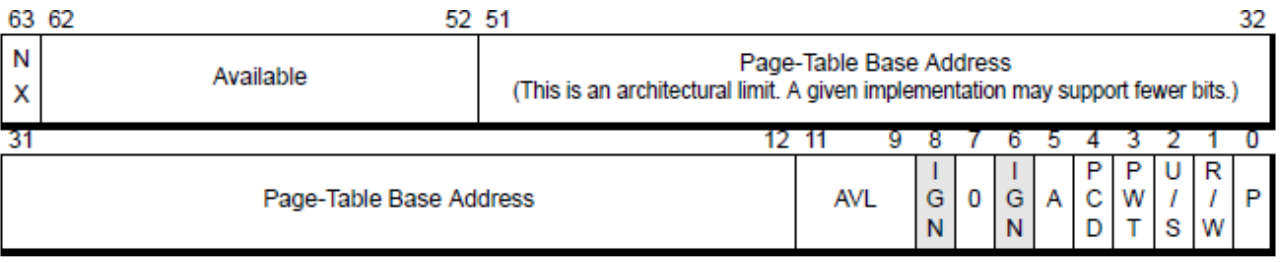
\includegraphics[width=0.8\textwidth]{21_i7L2.png}

\begin{description}
    \item[Page Table Phsyical Base Address:] $40$ MSB are the pointer to the base address of level 1
\end{description}

All other parts of the entry are equivalent to the previous levels.

\subparagraph{Level 1: Page Table Entry}
Is appointed by the page directory entry.

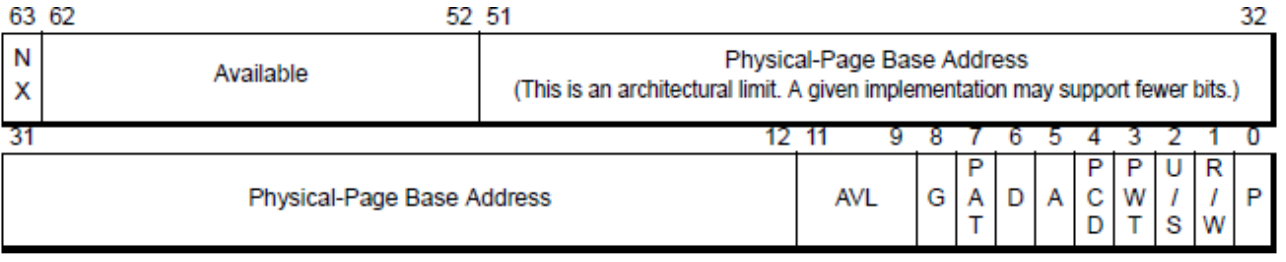
\includegraphics[width=0.8\textwidth]{21_i7L1.png}

\begin{description}
    \item[Phsyical Page Base Address:] $40$ MSB are the PPN
    \item[Avail:] Bits available to programmers for testing
    \item[G:] global bit
    \item[PAT:] page-attribute-table ???
    \item[D:] dirty bit
    \item[A:] access bit
    \item[PCD:] cache enable/disable bit
    \item[PWT:] write policy
    \item[U/S:] user/supervisor
    \item[R/W:] read/read-write
    \item[P:] present in memory flag 
\end{description}

\paragraph{Translation}
After the MMU receives the submitted VA, it splits it into the VPN and VPO parts. 

Firstly, the TLB is checked for a hit. 

\subparagraph{TLB Hit}
This is the ideal case for a translation.

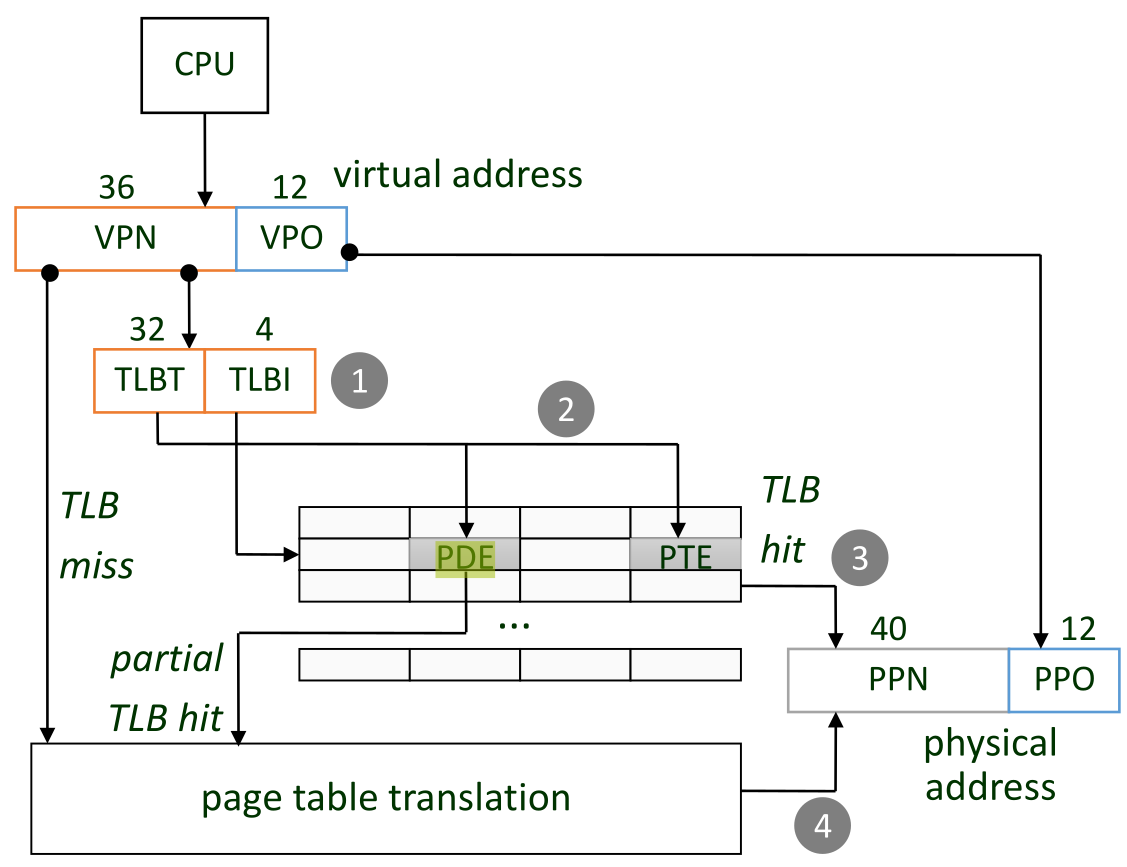
\includegraphics[width=0.8\textwidth]{21_i7TlbHit.png}

\begin{enumerate}
    \item The VPN is split again into TLBT and TLBI.
    \item The TLBI is used to index the table and simultaneously, the TLBT is used to check for matching layer entries.
    \item On a hit, the permissions are checked and if valid, the PPN is returned.
    \item If no TLBT matches (complete miss) or of not all tags of the $4$ entries matches (partial TLB miss), we have to get the missing data from the PT.
\end{enumerate}

\subparagraph{Page Translation (TLB miss)}
If we have a complete miss (none of the entries of the layers could be fetched) or a partial miss only some of the layer entries could be fetched), we have to page walk to get the PPN.

In the first example, all page tables as well as the page itself are present in memory. The MMU builds the physical address and can fetch the real data. This does not require any OS action.

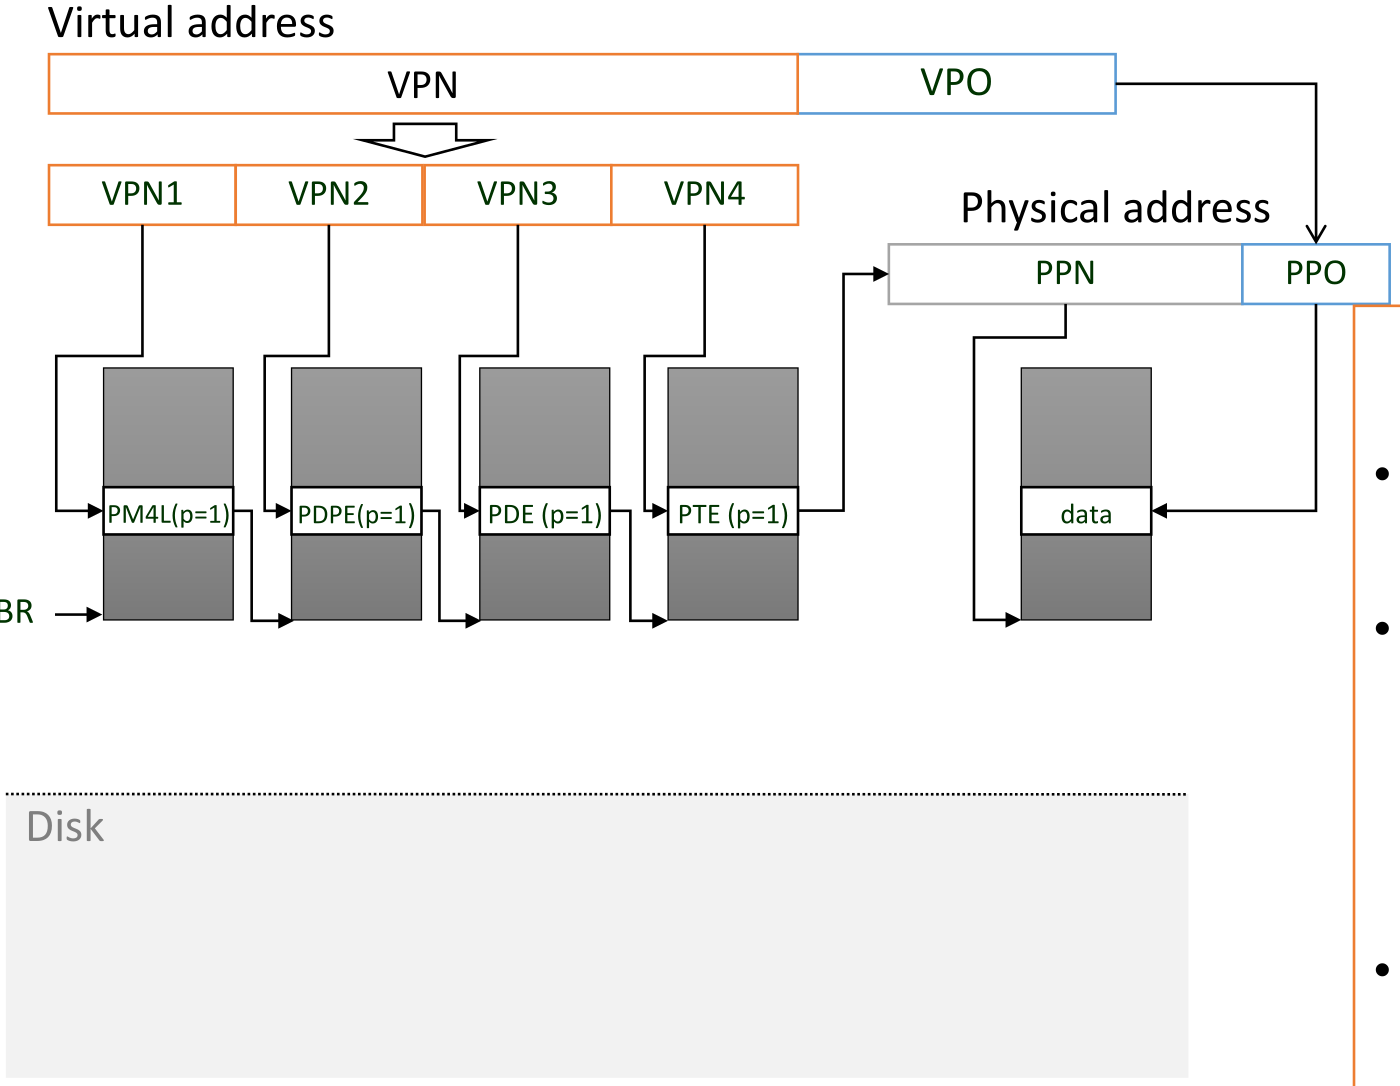
\includegraphics[width=0.8\textwidth]{21_i7Paging1.png}

In case that the page tables are present in memory but the page itself is in disk, de MMU triggers a page fault exception. The handler (OS) checks if the VA is legal and reads the PTE through the PT. It find free physical space and reads the VP from disk into the physical page. Then the handler adjusts the PTE to point to the PPN and sets the P flag to true. Then the faulty instruction is restarted.

The page fault exception handler may not only be triggered on \textit{non-present pages}, but also by \textit{page-level protections}. The so called \textit{Fault type}, is also given to the handler such that it knows the problem and can take appropriate action.

When one or multiple page tables as well as the page are missing, the MMU causes an page fault. As in the previous case, the OS brings the required data into memory, adjusts all flags and restarts the faulty instruction. Since this requires multiple consecutive disk reads, this is very expensive.

It may also happen that one ore multiple page tables are missing, but the page itself is present. This may introduce inconsistency issues and e.g. Linux disallows this.

\paragraph{Caches}
After the MMU translated the PA, we can check if the desired data is in cache.

First, the PA is split into CT, CI and CO. Using CI we index into the cached and check if we have a match using the CT. If we no not have a match the same procedure is repeated for L2, L3.... If we have a match, the word at offset CO is extracted.

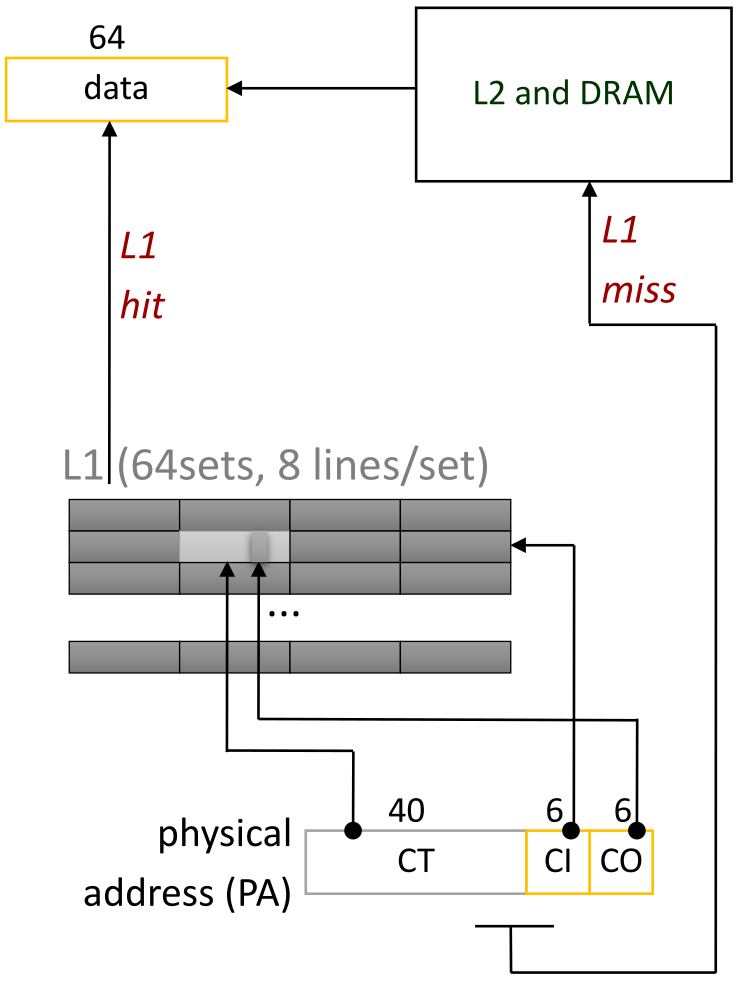
\includegraphics[width=0.8\textwidth]{21_i7Cache.png}

Even though L1 is rather fast, we can speed up the process even more. Since the CI is part of the PPO and hence does not change during the translation, we can start indexing the cache while address translation takes place. Since TLB hits most of the time, the PPN and with that also the CT bits get available rather quickly to validate cache matches.

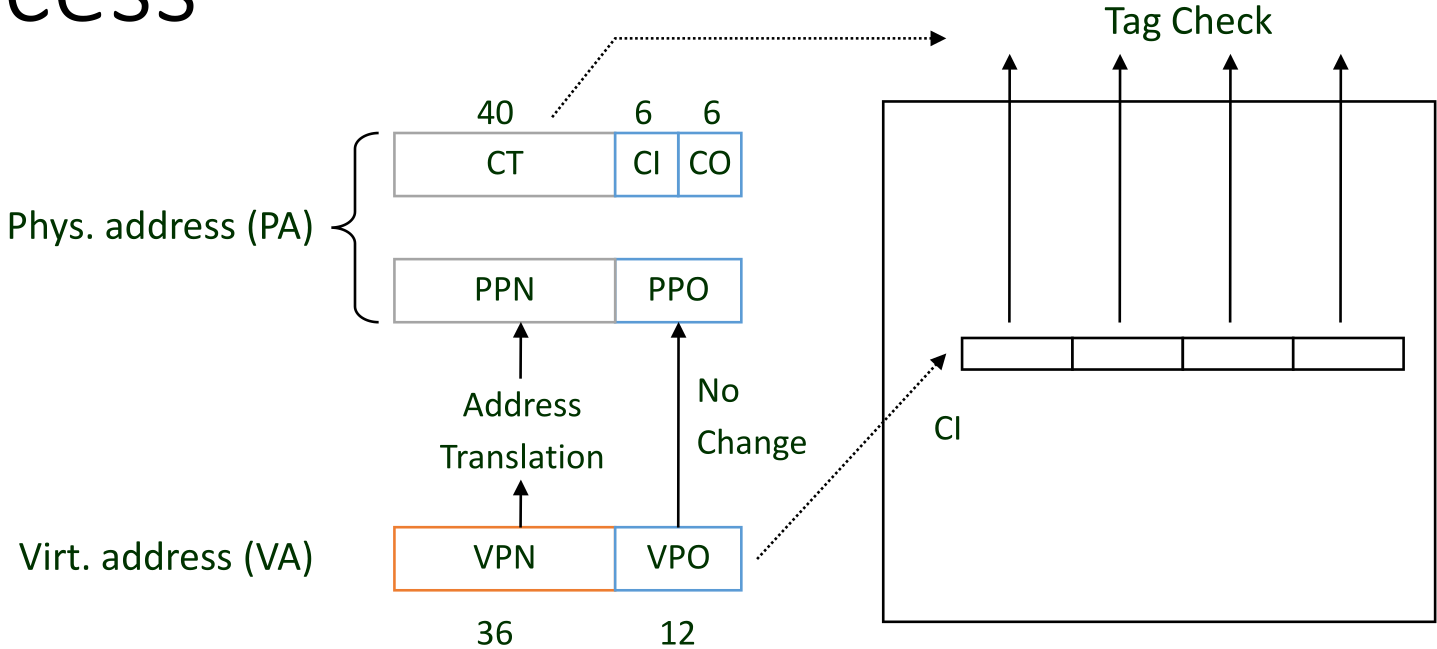
\includegraphics[width=0.8\textwidth]{21_i7CacheSpeedup.png}

\subsubsection{Cache Addressing}
Cache can be addressed using any combination of virtually/physical index and tag. The addressing also often differs for L1, L2 and L3.

\paragraph{Virtuall Indexed, Virtually Taged (VV)}
VV is also called virtually addressed cache and it can operate concurrently with the MMU. This makes it the fastest of all schemas for retrieving data.

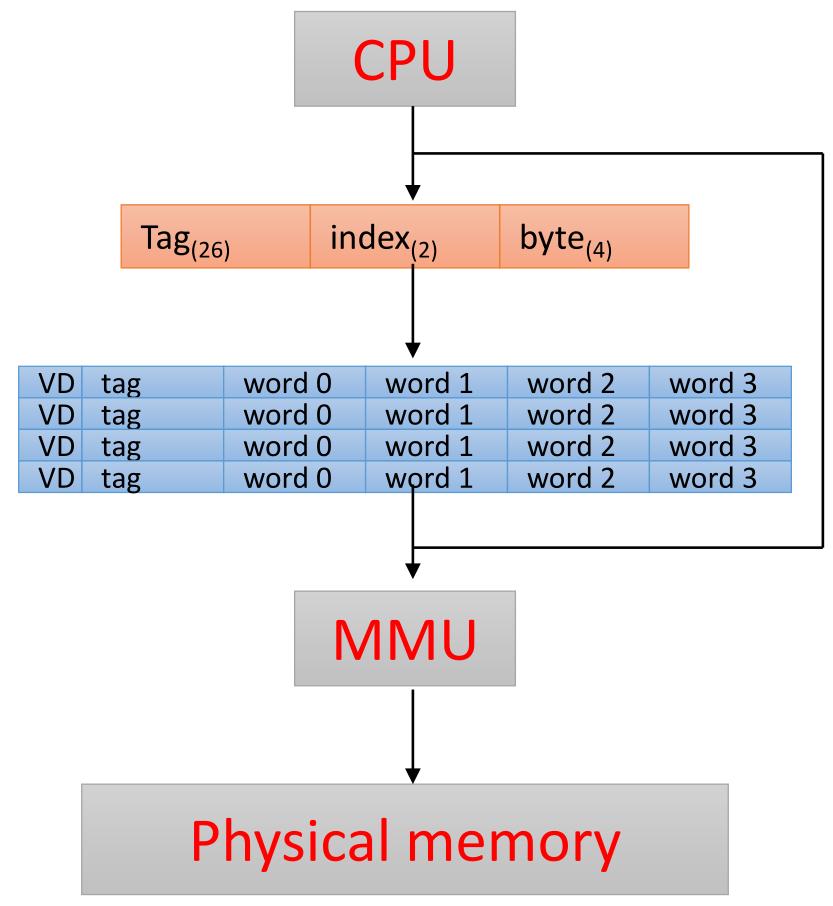
\includegraphics[width=0.8\textwidth]{21_CacheVv.png}

The main problem with this schema is \textit{homonyms}. The same VA refers different PAs for different processes. So, the tag does not uniquely identify data which leads to problems when trying to get data from the cache. Two simple fixes would be to flush the cache on context switch or to force non-overlapping address space layouts. A more reasonable solution is the tag the VA with a \textit{address space ID (ASID)}. On each access, the ASID of the cache is compared with the one of the process.

This resolved homonyms but leads to \textit{synonyms}. Different VAs map to the same PA. Therefore, we may have the same page in cache multiple times.

Another problem is caused by the write-back, then his schema requires a TLB lookup on writebacks in order to get the address to write to.

\paragraph{Virtually Indexed, Physically Tagged (VP)}
In this schema the VA gives the CI and the PA the CT. A smart implementation using alignment is required to prevent homonyms. This schema is commonly used for L1 caches.

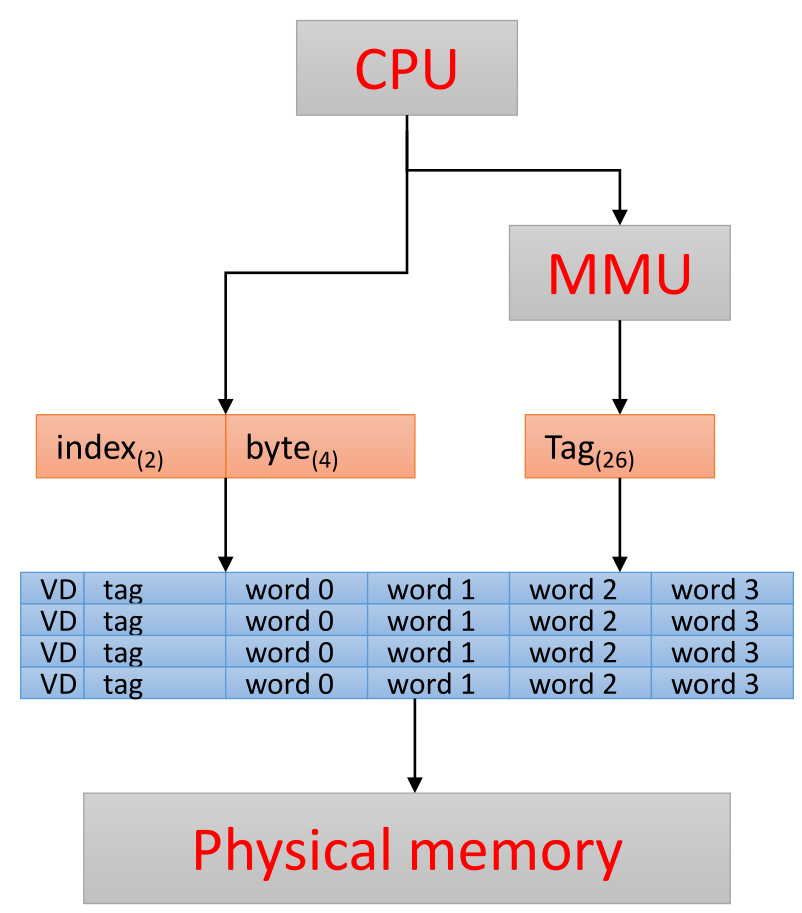
\includegraphics[width=0.8\textwidth]{21_CacheCp.png}


\paragraph{Physically Indexed, Virtually Tagged (PV)}
This schema is a bit pointless. If the PA has to be computed anyways we may easily also use the PA to get the CT.

\paragraph{Physically Indexed, Physically Tagged (PP)}
Since this schema only uses the PA, the PA has to be fully translated before we can start accessing the cache. This makes this type the slowest of all. But is is very simple to implement since there are no homonyms nor synonyms. This is often used for L2 or L3 caches.

\paragraph{Write Buffers}
Write operation take long time to complete. To avid stalling the CPU we can buffer writes on a FIFO \textit{Write Buffer} queue. It also allows for reading data from the queue to prevent stalling the CPU for reading data not yet written to disk. However, this makes the memory content temporarily stale. This gets especially tricky in multiprocessor systems.
